%\title{beavtex}
\documentclass[double,12pt]{beavtex}
\usepackage{graphicx}
\usepackage{rotating} %Package added to allow the rotation of figures and chart on a page, {sidewaysfigure} command
\usepackage{tablefootnote} %Packaged added to allow footnotes in the tabular environment, use \tablefootnote command
\usepackage{amsmath}
\usepackage{amsfonts}
\usepackage{color}



\title{Trabajo Pr\'actico N\'umero 1:}
\subtitle{"No creo que a \'el le gustara eso"}
\Agustina{Aldasoro, Agustina \ agusaldasoro@gmail.com}
\Belen{Bouz\'on, Mar\'ia Bel\'en \ belenbouzon@gmail.com}
\Gustavo{Cairo, Gustavo Juan \ gjcairo@gmail.com}

\submitdate{4 de Septiembre de 2014}

\begin{document}
\maketitle
\mainmatter

%-------------------------INTRODUCTION-----------------------------

\chapter{Introducci\'on Te\'orica}


Hab\'iendonos sido dados:

\begin{itemize}
\item la ecuaci\'on del calor que modela de forma gen\'erica el comportamiento de la temperatura T en un punto (x,y) $\in$ $\mathbb{R}^2$ (Ponerlo en funcion) luego de haber consolidado un estado estacionario (figura 1.1)

\item las medidas de un hipot\'etico parabrisas bidimensional cuyos m\'argenes se sabe que mantendr\'an una temperatura constante de -100ºC 

\item y ciertas posiciones del mismo que ser\'an sometidas a una temperatura constante (tambi\'en conocida) aplicada por  una clase id\'ilica y mutante de filo an\'elidos llamados hirud\'ineos (com\'unmente conocidos como "sanguijuelas") 

\end{itemize}

nuestros desaf\'ios consisten en:

\begin{itemize}

\item Proveer un algoritmo que - a partir de la consideraci\'on de los datos reci\'en citados - aproxime la temperatura esperada en condiciones de estabilidad en una cantidad finita de puntos del parabrisas. 

\item Optimizar dicho algoritmo aprovechando los beneficios potencialmente provistos por la estructura del sistema de ecuaciones planteado.

\item Dise\~nar e Implementar una funci\'on algor\'itmica que garantice, a partir de la eliminaci\'on de la menor cantidad posible de sanguijuelas, la perdurabilidad del parabrisas (esto es, el resguardo de su punto cr\'itico a una temperatura inferior a los 235ºC).
\end{itemize}

Como punto de partida y linea de desarrollo que nos permita conseguir estos objetivos, haremos uso e implementaremos en C++ el Algoritmo de Eliminaci\'on Gaussiana, poniendo en discusi\'on posteriormente posibles modificaciones del mismo que permitan adecuarlo a diversos contextos y necesidades.

Dicho algoritmo transforma un sistema lineal Ax= b, A $\in \mathbb{R}^{nxn}$, en uno equivalente Ux=y - donde U es una matriz triangular superior - permitiendo aplicar posteriormente el algoritmo de sustituci\'on regresiva que culmina en la resoluci\'on total del sistema.

\begin{equation}
\frac{\partial^2T(x,y)}{\partial x^{2}}+\frac{\partial^2 T(x,y)}{\partial y^{2}} = 0.
\end{equation}


\textcolor{red}{Che, esto quiero ponerlo en recuadro y que diga "figura 1.1" queda re colgado si no... pero I couldn't figure out how =(}



%------------------------DESARROLLO--------------------------------

\chapter{Desarrollo}

\section{Planteo del Sistema de Ecuaciones}

{\color{red}Texto tentativo:
Al  comenzar a plantear un sistema de ecuaciones que pudiera resultar efectivo para la resoluci\'on de los problemas presentados, se puso en cuesti\'on inicialmente el que se desarrolla a continuaci\'on:

Considerando la ecuaci\'on (la de la sumatoria y el promedio: $ t_ij$= blabla) pensamos que podr\'iamos diseñar una matriz que tuviera para cada i,j una ecuaci\'on asociada en funci\'on de las otras posiciones y que estuviera extendida con cada valor de $t_ij$ en el vector independiente. R\'apidamente descartamos esa posibilidad, ya que nos encontr\'abamos situando en el vector de t\'erminos independientes, varios que eran ciertamente dependientes.

Luego volvimos a la ecuaci\'on de la que hab\'iamos partido, que nos indicaba la propiedad que inexorablemente cumpl\'ia el comportamiento de la temperatura en funci\'on de la posici\'on consultada  y de la distribuci\'on de las sanguijuelas.  Le restamos a ambos lados $t_ij$ y obtuvimos una nueva expresi\'on igualada a cero, que determinar\'ia finalmente la estructura de nuestro sistema de ecuaciones, dado por:

	Sum(blablabl) –4 $t_iJ$= 0 para todos aquellos puntos que no tienen una temperatura constante (es decir, no pertenecen al borde del parabrisas ni se encuentran ocupados por sanguijuelas)



	$T_iJ$=-100 para todos los puntos del borde

	$T_ij$= $T_s$, siendo $T_s$ la temperatura aplicada por las sanguijuelas.
}




Frogs are weird...

\begin{figure}[ht!]
\begin{center}
	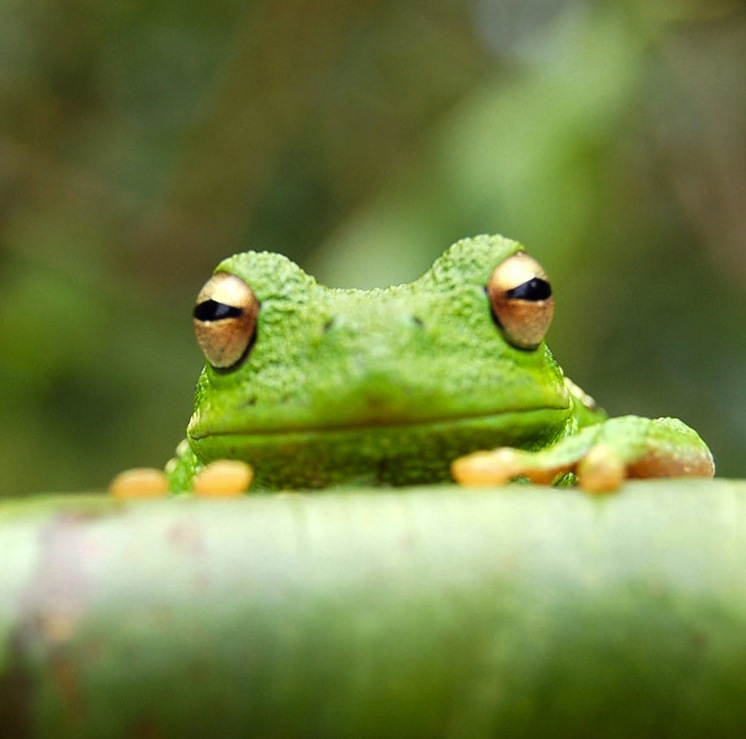
\includegraphics[width=9cm]{frog.jpg}
	\caption{Frog pic...}
	\label{fig:frog}
	\end{center}
\end{figure}


Here is a reference to the from pic: Figure~\ref{fig:frog}.

\section{Planteo acerca de las estructura internas de las matrices}

 Aca iria como armamos con arrays de arrays la matriz completa y como decidimos guardar la que es banda. Hay algo q ya escribi sobre esto, pero dado que considero que ustedes la tienen mucho mas clara con el codigo, me gustaria muchisimo q alguno lea lo escrito con mucha atencion y complete con lo que le parezca necesario recalcar en estas secciones. \\

{\color{red}Texto tentativo: \\
En cuanto al almacenamiento de nuestra matriz, al considerar su morfolog\'ia nos pareci\'o una idea plausible la de representarla almacenando  \'unicamente los elementos de la diagonal, los de la banda y los t\'erminos independientes. Gr\'aficamente:

[Dibujo de una matriz banda]

[Dibujo de lo q se guarda: sin los ceros intermedios]

Posteriormente nos dimos cuenta de que nuestra estructura podr\'ia traernos serios inconvenientes al momento de utilizarla como par\'ametro en el algoritmo de eliminaci\'on gaussiana e intentar hallar la soluci\'on al sistema, dado los ceros que se encuentran a la derecha de la diagonal y a la izquierda del fin de la banda son potencialmente modificables durante este procedimiento, y dichos cambios ser\'ian imperceptibles a pesar de ser determinantes a la hora de hallar la soluci\'on del sistema.

Ejemplo: 

[Me gustar\'ia poder poner una serie de pasos de triangulaci\'on en el q pase eso con un esquema de matriz propio del problema ]



Considerando este inconveniente, se resolvi\'o que una opci\'on que nos permitir\'ia optimizar el algoritmo de eliminacion gaussiana aprovechando la estructura de las matrices banda era la de almacenar de para cada fila el elemento de la diagonal, los dos elementos distintos de cero que se encuentren a su izquierda y tantos de los que se encuentren a su derecha como cantidad de columnas tenga la discretizaci\'on. [est\'a bien esto? Me gustar\'ia q lo pongamos con sub\'indices en vez de explicarlo tan feamente...]

Todavia faltaria decir que asi NO se guardo.. sino q volvimos a guardar los de la izq tambien}

\section{Planteo en relaci\'on al empleo de nuestras estructuras en el problema presentado}{
{\color{red}
\begin{itemize}
 \item Creo que deberiamos incluir lo que en el informe que les mande esta escrito como "Detalle sobre la ubicacion de las constantes en la matriz de las temperaturas" (creo q ni siquiera esta bien ponerle ese titulo porque habla sobre la matriz de posiciones principalmente... de como ubicar las sanguijuelas. o no? Me maree jajaja). Txt a continuacion: \\
Al momento de recibir por par\'ametro las posiciones de las sanguijuelas, nuestra matriz deb\'ia adaptar sus valores de acuerdo a la posici\'on de cada una de ellas, que podr\'ian alcanzar a ocupar un punto del parabrizas discretizado, varios o ninguno de acuerdo al radio, su centro y la medida de la discretizaci\'on escogida. 

Lo primero que dedujimos es que, llamando a h la discretizaci\'on, no se ver\'ia obligado a modificarse ning\'un punto que se encontrara a mayor distancia del centro (c) de la sanguijuela que el cuadrado determinado por los segmentos [escribir las formulas de los 4 segmentos del cuadrado]. De hecho, s\'olo lo estar\'ian dentro de aquella figura los que cumplieran$ (c_x-m_x)^(c_y-m_y)^2<=r^2$

-Explicar que primero hab\'iamos pensado la f\'ormula con sqrt pero nos pareci\'o q por la aritm\'etica finita aumentaba la probabilidad de error as\'i que tomamos el cuadrado. Experimentar con eso y evaluarlo cuando nos toque hacerlo.

Ponemos que otra idea fue que si el radio que te pasan es mas chico que la discretizacion que te pasan, exigirle al usuario otra discretizacion 

\item  Discusi\'on (¿?) sobre c\'omo calcular la temperatura en el punto cr\'itico cuando el mismo no se mapea a ning\'un punto de la discretizaci\'on: se usa la temperatura del m\'as proximo? El promedio de los cuatro q lo rodean? (acordarse q existe el caso en q los puntos mas cercanos no tienen nada pero tomando una grilla mayor es posible que la temperatura aumente considerablemente)


\item Problema si la sanguijuela no cae en ningun punto de la discretizacion pero esta muy cerca del critico: no se cuenta?Insert … Grafico del puntito rodeado. Culpamos a la discretizacion? Hacemos promedio? Calculamos una discretizaci\'on “m\'inima aceptable” relacionada al radio y la temp de las sanguijuelas? (no olvidarse q si esta cerca del bordepero tiene 8000 grados,elcentro esta al muertisimo igual.
\end{itemize}
}



\section{Planteo en relaci\'on a la implementaci\'on del Algoritmo de Eliminaci\'on Gaussiana y back substitution}
{ \color{red}
\begin{itemize}
\item{A la hora de pensar maneras de optimizar el c\'omputo de los c\'alculos vinculados a la matriz, tomamos en cuenta la posibilidad de considerar posibles particiones de la misma que reflejen patrones que pudieran repetirse, de modo que los mismos pudieran ser resueltos algor\'itmicamente una \'unica vez para luego replicar su resultado en m\'as de una oportunidad. Concluimos, finalmente , que este mecanismo resultar\'ia aplicable s\'olo en casos muy espec\'ificos para los cuales no existe ning\'un indicio de que su probabilidad de ocurrencia pudiera ser significativa}

\item Explicar c\'omo podr\'iamos haber cambiado el algoritmo de e.g. con pivoteo total (buscando el m\'aximo cada vez) para minimizar el error. Detallar c\'omo lo logramos sin eso, calcular cu\'al ser\'ia la complejidad de haberlo hecho. (para justificarnos, ja) Habria que poner que no lo usamos porque en este caso no nos cambia nada.

\item Demostrar LI de la discretizacion para justifcar la implementacion anterior edl algoritmo (en la q diagonalizabamos) probar que jamas podia pasar q se hiciera cero.

\item Antes dividiamos toda la fila por el coeficiente principal, para ya diagonalizar al principio . Esto acarreaba error porque hacia menos exacta la cuenta ya que no solo, se dividia al vector resultado sino que tambien a los demas coeficientes. 

Por lo tanto decidimos ir triangulando superiormente, y cuando quedaba la fila diagonalizada, dividirla por el coeficiente y asi va quedando la identidad igualada a su resultado. De este modo, se puede despejar las filas superiores con el resultado obtenido debajo.

Hacer una referencia a la seccion de experimentaciones y hacer ah\'i alguna comparando el algoritmo viejo y el nuevo y como queda menos exacto el calculo, al hacer mas divisiones innecesarias.

\item 
Problema con laresolucion de la matriz una vez triangulada: para despejar trabajo muchas mas veces sobre cada linea si triangulo normalmente que si despejo. C\'omo qued\'o al final? Estuve pensando, y creo que se trabaja lo mismo. Y da lo mismo, pero no se. Habria que charlarlo

\end{itemize}
}


%-------------------RESULTADOS--------------------------

\chapter{Resultados}

Cito: \\

Deben incluir los resultados de los experimentos, utilizando el formato mas adecuado
para su presentacion. Deber´an especificar claramente a que experiencia corresponde
cada resultado. No se incluir´an aqu´ı corridas de maquina\\
No es aceptable incluir tablas de resultados numericos siempre que sea posible su
graficacion. 
Esto no significa que se deban mostrar los resultados exclusivamente en forma de graficos.
Se debe buscar la manera de mostrar la informacion importante en la mejor forma de visualizacion. Este hecho sera tenido en cuenta para la evaluacion de la presentacion de los informes.
Es conveniente que el proceso de experimentacion no se realice en forma independiente
de la presentacion de los resultados, de manera que los resultados parciales obtenidos en
los primeros experimentos vayan orientando la experimentacion posterior.




\begin{table}[ht]
\caption{Types of stuff you put in a table} % title of Table
\centering  % used for centering table
\begin{tabular}{c c} % centered columns (2 columns)
\hline\hline                        %inserts double horizontal lines
Header 1 & Header 2 \\ [0.5ex] % inserts table heading
\hline                  % inserts single horizontal line
Item 1 & something  \\ % inserting body of the table
Item 2 & something else  \\
Item 3 & more things  \\
Item 4 & and more \\
Item 5 & last thing \\ [1ex]      % [1ex] adds vertical space
\hline %inserts single line
\end{tabular}
\label{table:misc} % is used to refer this table in the text
\end{table}





%------------------------DISCUSION--------------------------------

\chapter{Discusi\'on}

Cito: \\

Se incluira aqui un analisis de los resultados obtenidos en la seccion anterior (se analizara
su validez, coherencia, etc.). Deben analizarse como mınimo los items pedidos en el
enunciado. No es aceptable decir que “los resultados fueron los esperados”, sin hacer
clara referencia a la teorıa a la cual se ajustan. Ademas, se deben mencionar los resultados interesantes y los casos "patologicos" encontrados.

La seccion de discusion debe estar relacionada indefectiblemente con el desarrollo y los
resultados presentados en las secciones anteriores. No se aceptaran afirmaciones que no esten
respaldadas por los datos presentados


\begin{equation}
MDC=\frac{3.29*\sqrt{(Bkgcpm*C_{t}*(1+\frac{C_{t}}{BkgC_{t}}))}+3.0}{2.22*E*C_{t}*V*decay*A*R*DF*I}
\label{eq:mdc}
\end{equation}
Where:

\begin{itemize}
\item $C_{t} =$ Sample count time
\item $BkgC_{t} =$ Background count time
\item $Bkgcpm =$ Background counts per minute (cpm)
\item $E =$ Counting efficiency
\item $V =$ Sample volume or weight
\item $decay =$ isotopic decay (if applicable)
\item $A =$ Isotopic abundance (if applicable)
\item $R =$ Recovery (if applicable)
\item $DF =$ Dilution factor for liquid scintillation (if applicable)
\item $I =$ Additional decay or ingrowth factors (if applicable)
\end{itemize}




\pagebreak[4]

\begin{figure}
\begin{center}
	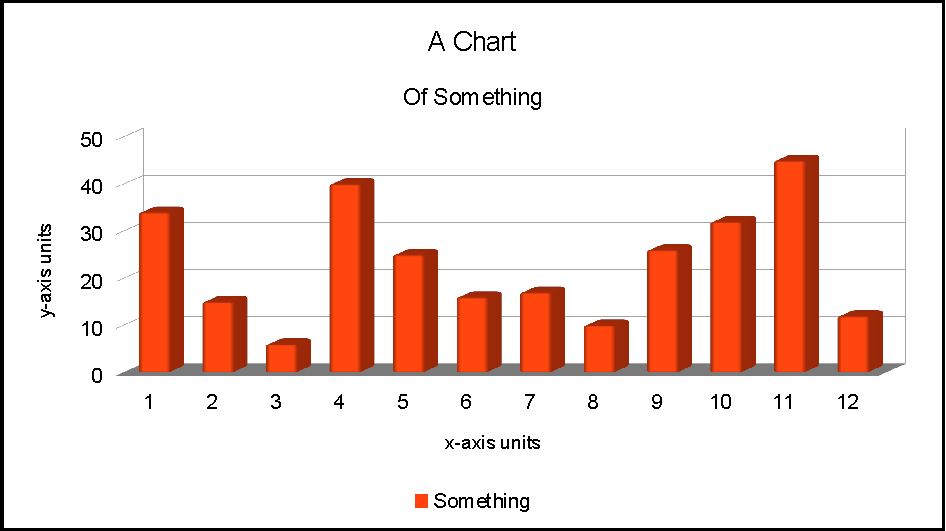
\includegraphics[width=14cm]{chart.pdf}
	\caption{A Chart.}
	\label{fig:chart}
	\end{center}
\end{figure}

\pagebreak[4]

\begin{sidewaysfigure}[htbp]
\begin{center}
	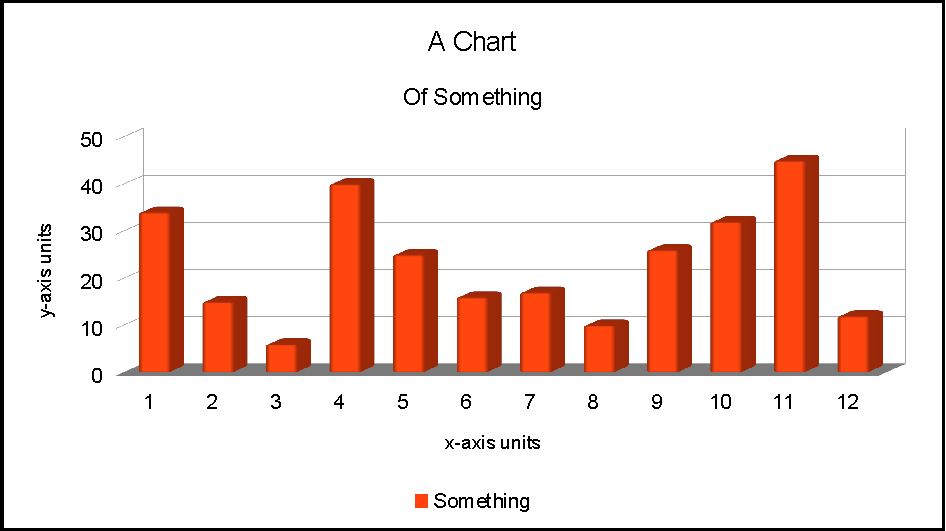
\includegraphics[width=18cm]{chart.pdf}
	\caption{Same chart, but using sidewaysfigure.}
	\label{fig:rain}
	\end{center}
\end{sidewaysfigure}


%-----------------------CONCLUSION--------------------------------

\chapter{Conclusiones}

Cito: \\

Esta seccion debe contener las conclusiones generales del trabajo. Se deben mencionar
las relaciones de la discusion sobre las que se tiene certeza, junto con comentarios
y observaciones generales aplicables a todo el proceso. Mencionar tambien posibles
extensiones a los metodos, experimentos que hayan quedado pendientes\\
Se pide certeza y rigor logico de la discusion, el analisis y las conclusiones. Se pondra especial
enfasis en que las conclusiones se desprendan de las experiencias realizadas. 

\section{First Subsection}

FRUTA 

\begin{equation}
A(t)=A_{o}e^{(-\lambda t)}
\label{eq:initialeq}
\end{equation}

Then Equation~\ref{eq:initialeq} is integrated to become:

\begin{equation}
\tilde{C}=\int_0^{t}A(t)dt = \frac{A_{o}}{\lambda} (1-e^{(-\lambda t)})
\label{eq:finaleq}
\end{equation}

Where:

\begin{itemize}
\item $A(t) =$ original exponential function
\item $A_{o} =$ the peak activity at day 0 (Bq per mass or volume)
\item $\tilde{C} =$ Integrated Activity Concentration (Bq-days per mass or volume)
\item $t =$ 28 days
\item $\lambda =$ removal constant (day$^{-1}$)
\end{itemize}


Finally, a table with a footnote...

\begin{table}[htbp!]
\caption{Some table values}
\centering
\begin{tabular}{cccccc}
\hline\hline
 & & & & & Total \\
Sample & $A_{o}$\tablefootnote{some kind of footnote from a table, which doesn't work without the tablefootnote package} & $\lambda$ & $\tilde{C}$ & Something & (units) \\
\hline   \\
Item 1 & 1 & .55 & 3 & 125 & 70  \\
Item 2 & 1 & .55 & 3 & 125 & 70  \\
Item 3 & 1 & .55 & 3 & 125 & 70  \\
Item 4 & 1 & .55 & 3 & 125 & 70  \\ [1ex]
\hline
\textbf{Total} &  &  &  &  & \textbf{280} \\ [1ex]
\hline
\end{tabular}
\label{table:intake2}
\end{table}






\chapter{Ap\'endices}

\section{Ap\'endice A}

Ac\'a va el enunciado del TP, pero no pude copiarlo y pegarlo directamente xq incluye cosas locas.

\pagebreak

\section{Ap\'endice B}

Ac\'a van codigos fuente de funciones relevantes desde el punto de vista numerico (?) 

\section{Ap\'endices con numeros romanos}
resultados que valga la pena mencionar pero que sean demasiado especificos como para aparecer en el cuerpo principal. X ej una demo de una propiedad que aplicamos para optimizar el algoritmo

\bibliography{thesis}

\chapter{Referencias}
\bibliographystyle{plain}

\pagebreak







\end{document}